\documentclass[12pt]{article}

% Packages
\usepackage[margin=1in]{geometry}
\usepackage{setspace}
\usepackage{times}
\usepackage{amsmath}
\usepackage{booktabs}
\usepackage{array}
\usepackage{tabularx}
\usepackage{graphicx}
\usepackage{hyperref}
\usepackage{tabularray}
\UseTblrLibrary{booktabs}
\UseTblrLibrary{siunitx}
\usepackage{caption}
\usepackage{siunitx}
\usepackage{float}
\usepackage{microtype}
\setlength{\parindent}{2em}
\setlength{\parskip}{0pt}
\usepackage[style=apa, backend=biber]{biblatex}
\addbibresource{references.bib}
\doublespacing

\hypersetup{
    colorlinks=true,
    linkcolor=black,
    citecolor=black,
    urlcolor=blue
}

% Title info
\title{Authoritarian Intergovernmental Organizations and Amendment Flexibility}
\author{}
\date{}

\begin{document}

\maketitle

\begin{abstract}
Conventional wisdom holds that authoritarian regimes resist institutional flexibility in international organizations, favoring unanimity rules to preserve veto power. This article challenges that assumption by theorizing the conditions under which autocracies prefer majoritarian amendment rules. I argue that when embedded in intergovernmental organizations (IGOs) composed largely of fellow autocracies, authoritarian states are more willing to forgo veto power than democracies. Shared regime interests, particularly around sovereignty, non-interference, and political stability, reduce both the ideological distance among members and the domestic political costs of implementing unwanted amendments. Using a dataset of IGOs from 1950 to 2014, I find that clubs of autocracies are significantly more likely to adopt majority-rule amendment procedures, instead of unanimity, than their democratic counterparts.

\medskip
\noindent\textbf{Key words:} Intergovernmental Organizations, International Law, Rational Design of Institutions, Voting Rules, Authoritarianism
\end{abstract}

\newpage

\section{Introduction}

Can authoritarian state leaders tolerate institutional flexibility? Autocratic states are widely assumed to resist ceding veto power in international organizations, preferring unanimity rules and rigid procedures that shield them from unwanted policy change. This paper complicates that assumption. I argue that an authoritarian state's willingness to forgo veto power depends on the regime composition of the organization. Once we bring our attention to authoritarian states' decisions with regards to clubs of fellow autocrats, it opens the possibility of cohesive cooperation through veto waivers. Drawing on theories of institutional design, I show that authoritarian leaders incur lower domestic political costs when implementing collectively decided amendments among like-minded peers.

Throughout this manuscript, I conceptualize amendment flexibility as the degree to which an IGO's founding treaty can be revised through lower voting thresholds and minimal ratification constraints. Flexible amendment rules through simple majority voting allow IGOs to adapt more readily to changing circumstances but reduce individual states' control over constitutional change. In contrast, unanimity requirements grant each member de facto veto power, thereby maximizing control but reducing flexibility \parencite{lutz_toward_1994, ferejohn_politics_nodate}.

This paper joins the literature on institutional design by introducing an interaction between regime type and IGO design choices. Recent research on authoritarian international cooperation suggests that autocratic states are increasingly building their own formal institutions, coupled with codified treaties and bureaucratic organizations that can reinforce regime durability and reduce democratization risks \parencite{debre_are_2025, debre_clubs_2022, cottiero_illiberal_2025, obydenkova_authoritarian_2019, ginsburg_authoritarian_2020}. 

Despite existing work on AIGOs' pooling and delegation at the aggregate level
\parencite{tallberg_democracy_2025}, and at specific domains such as dispute settlement
mechanisms \parencite{bae_regime-type_2025}, neither directly speaks to amendment
flexibility. \textcite{tallberg_democracy_2025} find that regime type predicts aggregate
pooling and delegation scores for general-purpose IGOs, but their aggregate index combines
constitutional amendment rules with routine policy voting, membership procedures, and
other institutional features into a single score. It is therefore an open empirical
question whether the regime-type effect they identify is driven by amendment procedures
specifically, or by other components of the index. This distinction matters because
amendment rules carry a qualitatively different political logic. Unlike routine policy
decisions, constitutional revisions alter the foundational rules of the organization
itself and are far more difficult to reverse. A state's calculus over whether to accept
majority rule for day-to-day decisions may differ substantially from its calculus over
permanent constitutional change. Disaggregating the aggregate index to isolate amendment
flexibility is therefore not a replication of \textcite{tallberg_democracy_2025} but a necessary next step to determine which institutional domain is actually driving their
result.

To preview my argument, when authoritarian states predominantly hold seats at IGOs, they are actually better positioned to give up veto power on amendments for IGOs' constitutive treaties compared to democracies for two reasons. First, it is expected that the deviation between amendment choices from the rest of the group and individual country will be minimal, since AIGOs tend to be homogeneous in terms of cautionary actions against potential democratization risk factors. Second, even when authoritarian states end up having to accommodate less desirable amendments, they can soften the blow by framing the issue to be less salient.

\section{Autocrats as Entrepreneurs of Global Governance}

In this section, I situate the theme of authoritarian states' cooperation through formal AIGOs along with codified constitutive treaties. To paint a clearer picture of what these clubs of authoritarian states look like, I introduce an illustrative case of Myanmar that shows how the ASEAN (Association of Southeast Asian Nations) Charter was invoked. As the following example will show, founding legal instruments take a substantial presence in the authoritarian playbook.

The former Myanmar's leader, Aung San Suu Kyi invoked the principle of non-interference in her favor amidst charges of genocide committed against the Rohingya Muslim minority. During the UN Security Council meeting, Myanmar expressed its gratitude toward members of the Security Council ``who upheld the principle of non-interference in the internal affairs of sovereign countries,'' and condemned liberal democracies' pressure as an act of infringement on sovereignty. When the topic of junta was broached, members of ASEAN invoked the principle of non-interference in the Charter and maintained a rather acquiescent stance, by calling the coup ``an internal affair'' that remains in Myanmar. Whether this rhetorical engagement is effective in persuading international audiences, it is nevertheless a popular strategy used by autocrats when they try to deflect criticism under the shield of international law with the interpretation that serves their political purposes.

It is not just an anecdotal case that intergovernmental projects with like-minded autocrats indeed directly help regime survival against democratization pressure. \textcite{von_soest_democracy_2015} points out that authoritarian coordination is driven by political motivations rather than commitment to ideologies, and is shown through patterns of selective support of one another. Recent literature on authoritarian international law has highlighted how autocracies are not merely passive recipients of international norms but are actively shaping legal frameworks to reflect their interests \parencite{ginsburg_authoritarian_2020}. In \textcite{debre_clubs_2022}'s seminal work, authoritarian state leaders who have been members of authoritarian clubs tended to survive longer in their incumbencies, everything else equal. In this sense, AIGOs and their constitutive treaties that enshrine the key principles of authoritarian cooperation are crucial tools for authoritarian survival, showing the substantive importance of treaty content and its amendments.

According to \textcite{hooghe_international_2017}, the constitution of an IGO refers to ``a set of fundamental principles or established precedents for the governance of an organization.'' For consistency, I use the term ``constitution'' to denote the organization's supreme law that publicly declares its foundational principles and goals. IGO constitutions take various names and forms. For example, some organizations are established through documents labeled ``Constitutive Instruments,'' ``Treaty,'' or ``Charter'' \parencite{hooghe_constructing_2017}. Regardless of terminology, the supreme law at the apex of an organization's legal framework is typically a constitutive treaty adopted at the IGO's inception. To clarify the paper's central focus, I examine whether IGOs composed of autocratic states adopt more relaxed rules for proposing and enforcing amendments to their constitutions.

\section{Theory of Authoritarianism and Amendment Flexibility}

Against this background, I unpack why AIGOs are more likely to favor flexibility around their constitutions. To do so, I focus on the political costs of majority rule and how regime type mediates these costs. Theories of rational institutional design and domestic constitutional change both emphasize how voting rules reflect states' expected benefits and legal culture \parencite{ginsburg_does_2015}. 

Yet, existing literature has not explored regime type as a mediating channel between voting rules and political costs that have to be paid at the domestic level. I briefly discuss the cost side of amendment flexibility. Specifically, I argue that authoritarian regimes are not only motivated by the benefits of flexible rules, but are also structurally better equipped to absorb their costs, especially the risk of being bound by undesired amendments.

Building on \textcite{buchanan_calculus_1965}'s model of collective decision-making, I define political cost as the domestic burden of readjusting policies or institutions to conform with a collectively adopted amendment that deviates from a state's preferred outcome. Because these costs are shaped by domestic political structures, regime type helps explain why some states can afford to relinquish veto power while others cannot. This perspective extends existing theories that emphasize states' desire for flexibility under uncertainty by introducing affordability as a necessary condition for institutional design. While many regimes may prefer flexibility in principle, only some can bear its costs in practice. Focusing solely on demand overlooks this crucial constraint and cannot fully explain variation in amendment procedures. In what follows, I explain why authoritarian regimes, unlike democracies, are more capable of absorbing the domestic political costs that flexible amendment procedures entail.

\subsection{Why Authoritarian States Can Afford Flexibility}

Compared to unanimity rules, majority rule lowers the threshold for collective decision-making and enables greater institutional flexibility \parencite{posner_voting_2014}. But this flexibility comes at a price: States must relinquish veto power and accept the possibility of being bound by decisions they oppose. A country may find itself in the 49\% minority on a constitutional amendment and still be required to implement the outcome. AIGOs are better equipped to manage this risk because the domestic political costs of implementing undesired amendments are lower for autocratic leaders. Unlike democratic governments, which must navigate electoral accountability, legislative oversight, and interest group pressure, authoritarian regimes face fewer institutional constraints and weaker domestic channels of contestation \parencite{hollyer_why_2011}.

In contrast, state leaders of democracies are more likely to face domestic pushback when implementing international amendments that diverge from public preferences or partisan agendas, particularly in politically sensitive areas, facilitated by media \parencite{dai_why_2005, baum_relationships_2008}.Citizens in democracies even evaluate the legitimacy of international law as a whole rather than compliance per se \parencite[]{morse_smoke_2025}.   Empirical evidence from survey experiments show that citizens in democratic regimes tend to prefer foreign policies that align with international legal commitments their governments have ratified \parencite{wallace_international_2013, lupu_laws_2024}. As a result, while both authoritarian and democratic state leaders may recognize the benefits of amendment flexibility, only some can absorb the associated political costs. This asymmetry in domestic political vulnerability affords authoritarian IGOs greater latitude to adopt flexible, majority-rule amendment procedures.

To tighten the logic, I unpack the concept of political cost along two dimensions that align with institutional design choices: (1) the expected gap between a state's ideal point and the outcome of a majority-vote amendment, and (2) the domestic significance of implementing that undesired outcome. The first dimension captures how ideologically or strategically misaligned a given amendment is from a state's ideal point---greater misalignment increases the cost of compliance. The second dimension reflects how burdensome or politically risky the amendment is to implement at the domestic level, such as when it affects sensitive policy areas or challenges powerful interest groups. These two components jointly determine the perceived cost of flexibility. In the next section, I show that regime type conditions both dimensions: authoritarian regimes tend to face lower expected distance within ideologically homogenous IGOs and are better equipped to absorb the domestic impact of undesired decisions, making them more likely to tolerate majority-rule amendment procedures.

\subsection{Two Dimensions of Political Cost: Ideological Distance and Domestic Burden}

The first component of political cost is the expected distance between each authoritarian state's ideal policy point and deviating collective decision. The distance between the new constitution's pursuit and each member state's ideal point is expected to be small for member states of AIGO. With a homogeneous priority, authoritarian states do not expect the worst-case scenario of having an entirely new normative goal when they waive veto power for amendments.

To ground this assumption, I draw on empirical studies that document the internal coherence of AIGOs. AIGOs, composed primarily of authoritarian regimes, tend to exhibit greater alignment in core principles than their democratic counterparts \parencite{obydenkova_authoritarian_2019}. AIGOs are ideologically more cohesive around shared priorities like regime durability and insulation from external pressures that often come from liberal democracies \parencite{debre_are_2025}. As \textcite{ginsburg} shows, IGOs dominated by autocracies are more likely to explicitly enshrine principles of sovereignty and regime preservation in their founding documents. In contrast, IGOs led by democracies often emphasize liberal norms such as transparency and accountability, which can generate greater internal divergence. This internal coherence among AIGOs reduces the probability of ideologically misaligned amendments, thereby lowering the first major source of political cost associated with flexible amendment procedures.

A useful empirical case that illustrates this logic is the Shanghai Cooperation Organization (SCO). Founded by China, Russia, and several Central Asian states, the SCO reflects a high degree of ideological and institutional alignment among its authoritarian member states. From its inception, the SCO's charter and agreements emphasized mutual respect for sovereignty and non-interference, codifying the shared priorities of its members. This ex ante agreement on core values allowed member states to adopt progressive projects on high-stake domains like military cooperation. For example, through its Regional Anti-Terrorist Structure (RATS), the SCO conducts joint counterterrorism exercises and facilitates intelligence sharing and border security coordination among members.

The SCO's founding design was explicitly shaped by concerns about Western-led institutional models, and member states have shown little fear that internal amendments would threaten their domestic political orders. The case of the SCO therefore illustrates how authoritarian regimes design IGOs with the expectation of ideological proximity, which in turn reduces the perceived risks of majority-rule procedures and facilitates greater amendment flexibility.

The second element of political cost is the expected readjustment cost (both political and fiscal) of making domestic changes for a new amendment. States have to explain and justify why such a new direction is wanted and adjust domestic rules in ways that align with collective interests by setting up relevant bureaus. Authoritarian state leaders have greater leeway in both aspects. Leaders in autocracies often exercise control over legislatures, state media, and administrative agencies, allowing them to downplay, delay, or reinterpret external obligations with minimal political repercussions \parencite{dai_why_2005, weeks_autocratic_2008}.

Constitutional amendments bring about significant political ramifications on the ground. The ASEAN Charter, for example, has gone through multiple amendments, as collective gains to harvest were large and it provided enough incentives for members to invest resources to make amendments. Several amendments for the ASEAN Charter added more specific action plans like implementing the shared database of non-tariff measures, and accelerating free trade by removing non-traditional barriers \parencite{asean2004}. Some of the changes require a substantial amount of domestic effort, given the level of precision. Member states were expected to pay the economic cost of implementing new administrative task forces and the political cost of legitimating changes and appropriation of budget. The argument I'm making here is that these readjustment costs are significantly lower for authoritarian states than democracies.

To illustrate a short example of Thailand, one of the key members of the ASEAN, Prime Minister Yingluck Shinawatra during the administration in 2014 had to answer the question regarding amendments raised by a competing party leader about whether the country is prepared to manage free movement of laborers from ASEAN community given its dependence on agricultural and labor-intensive industries. The question was raised with a reference to the ASEAN Framework Agreement that specified a 5-year plan. There were several parliamentary debates before and after the ASEAN meeting, given the cost of political adjustments even for authoritarian states. But the degree to which such a political decision affected the approval rate was significantly low in this case.

In contrast, liberal democracies often face higher domestic political costs when engaging in IGO constitutional amendments, especially when proposed changes intersect with salient interest group divisions. A clear example is the 2005 rejection of the European Constitution by referendums in France and the Netherlands. Despite strong elite-level support and approval by the European Parliament, domestic constituents vehemently opposed the change, ultimately voting ``no.'' This resistance halted the constitutional initiative and forced the EU to pursue a revised treaty structure---the Lisbon Treaty---which also faced political hurdles in Ireland. These examples demonstrate how, in democracies, treaty amendments can become flashpoints for public backlash, compelling governments to renegotiate, delay, or abandon institutional reforms.

Together, these cases highlight that while both regime types must justify policy changes to domestic audiences, the political risks of failure are often higher in democracies, particularly when public ratification is required. At the extreme, democratic governments may even use international organizations as scapegoats to shield themselves from domestic criticism, especially when a dispute is highly salient \parencite{lim_why_2022}. More broadly, engagement with international institutions has become a growing source of polarization in many democracies. Of course, all leaders must navigate domestic constraints to some extent, but the magnitude and consequence of failing to justify institutional change diverge significantly across regime types.

In sum, authoritarian states are better positioned to adopt majority decision rules compared to democratic states. Their greater tolerance for sub-optimal outcomes and lower domestic political costs enable them to accept group decisions, even when these diverge from individual preferences. As a result, they are more willing to embed collective commitments into constitutional reform, facilitating flexibility. In the next section, I empirically evaluate this claim by examining whether AIGOs are more likely to adopt majority-rule amendment procedures. Specifically, I assess how variation in regime type across IGOs correlates with their constitutional design choices, with particular attention to the threshold required for treaty amendment.

\section{Data and Methods}

I use panel data of 76 IGOs from 1950 to 2014 drawn from the Measuring International Authority dataset \parencite{hooghe_constructing_2017}. This time scope captures the landscape of international governance beginning with the second democratization wave. To measure member states' regime type, I use the polyarchy index from the Varieties of Democracy project \parencite{vdem_codebook_2023}, which provides a continuous 0 to 1 scale capturing electoral competitiveness and participation. Compared to binary democracy measures, polyarchy allows for finer-grained comparisons across countries and over time, making it well suited to assessing IGO membership composition. I supplement the MIA dataset with the Correlates of War IGO data (2019) to obtain organizational characteristics, including whether an IGO pursues general or task-specific goals. This ensures the sample excludes ad hoc alliances and informal groupings that lack enduring institutional structure.


\subsection{Measurement of Amendment Flexibility}

To operationalize the main dependent variable, amendment flexibility, I use the ``constitutional pooling'' score from the MIA dataset. This score captures the extent to which member states delegate authority to collective decision-making processes when it comes to revising an IGO's constitution. While this indicator captures formal (de jure) flexibility rather than the frequency of amendment in practice, it aligns closely with the theoretical focus of this study---the willingness of states to design institutions that allow for constitutional change without unanimity. By measuring how much discretion states forgo ex ante in institutional design, constitutional pooling serves as a valid and theoretically consistent proxy for amendment flexibility.

The score is constructed as a voting rule weighted by ratification constraints, as shown in Table~\ref{tab:pooling}. Constitutional pooling increases as decision rules move closer to simple majority and away from unanimity. The more ratifications required to implement an amendment, the lower the pooling score, even when majority voting is formally adopted. The Gulf Cooperation Council, for example, requires unanimity for amendments but no ratification, so the amendment takes effect automatically once passed. The League of Arab States uses a two-thirds majority rule but requires ratification, giving members substantial latitude to opt out. The average constitutional pooling score across the sample is 0.209, indicating that most IGOs fall well short of full majority rule.

\begin{table}[H]
\centering
\caption{Two Components of Pooling on Constitutional Reform}
\label{tab:pooling}
\small
\begin{minipage}{0.38\textwidth}
\centering
\begin{tabular}{lc}
\toprule
\textbf{Voting Rule} & \textbf{Score} \\
\midrule
Individual members decide & 0 \\
Unanimity & 0.33 \\
Supermajority & 0.66 \\
Simple majority & 1 \\
\bottomrule
\end{tabular}
\end{minipage}
\hspace{0.2em}
\begin{minipage}{0.60\textwidth}
\centering
\begin{tabular}{lc}
\toprule
\textbf{Ratification Requirement} & \textbf{Score} \\
\midrule
Ratification required by all & 0.25 \\
Ratification required by a subset, result binding on subset & 0.50 \\
Ratification required by a subset, result binding on all & 0.75 \\
No ratification required & 1.00 \\
\bottomrule
\end{tabular}
\end{minipage}
\end{table}

What does it look like for an IGO to completely pool decision making power around constitutional revision? Under this scenario, member states forgo veto power and lower the bar for passing amendments to simple majority. Yet, pooling means something more than a simple voting rule. One important factor of decision making in the international realm is that the decision outcome possesses little to limited power if every member's ratification at domestic level is required for the amendment to come into effect. The ratification clause requires that international decisions be domestically approved in member states' legislation. It can practically nullify a new amendment that has been approved with unanimity rule. Existence of ratification requirement thus decreases pooling score, even when the group chooses majority voting rule.

Constitutional pooling score increases as a decision rule for amendment gets closer to majority rule, further from unanimity rule. Simple majority decision rule gets a higher pooling score than two thirds, and unanimity rule (consensus). In addition, the more ratifications an IGO needs to fully implement the amendment, the less score it gets on pooling. The Gulf Cooperation Council, for example, employs the unanimity rule for new amendments to the Charter of the Gulf Cooperation Council. Although the GCC requires unanimity, ratification isn't required and once the amendment passes, it's automatically in action. In the case of the League of Arab States, even though two thirds majority voting rule is employed for constitutional amendments, ratification is required which gives way more latitude for members to opt out by not ratifying it. Pooling score is an inversely weighted voting rule with respect to ratification requirements.



To measure the level of democracy of an IGO, instead of a single country, I constructed the IGO-level democracy score by formulating the average polyarchy score of all the member states for each IGO in a given year. Additionally, I measured member states' heterogeneity in terms of their regime types by using standard deviation of members' polyarchy scores. This proxies a distribution of political disparity among member states at an IGO level. 


To directly operationalize observable heterogeneity seen among one another, I created another variable, preference heterogeneity, that is based on standard deviation of ``state ideal points'' from the United Nations General Assembly voting results \parencite{bailey_estimating_2017, voeten_clashes_2000}. Since voting results are publicly available to state representatives, this variable offers a good way of measuring ``perceived'' compatibility in policy directions and preferences among member states. \textcite{bailey_estimating_2017} estimated ideal points using the UNGA voting data that are comparable across time and issue areas.

There is no a priori reason to expect that authoritarian states cooperating in formal IGOs would exhibit greater preference dispersion than their democratic counterparts. Authoritarian states that choose to build institutions together do so precisely because they share core priorities around sovereignty, non-interference, and regime preservation \parencite{obydenkova_authoritarian_2019, debre_are_2025}. The sorting mechanism itself generates cohesion as a byproduct in that states that deeply disagree on foundational principles do not build formal organizations together in the first place \parencite{mansfield_democratization_2006, tallberg_democracy_2025}. Figure~\ref{fig:homogeneity} demonstrates this empirically. Preference heterogeneity follows a pattern across the democracy spectrum, peaking among mixed IGOs near the 0.5 threshold and declining sharply at both extremes. Purely authoritarian IGOs exhibit the lowest preference dispersion in the sample, consistent with the expectation that ideological sorting produces cohesive clubs at the authoritarian end of the spectrum.


If members are heavily reliant on international trade, then an IGO is expected to have a higher level of pooling as domestic interest groups ask for more cohesive cooperation across the borders to facilitate trade. Trade variable is an average score of total trade volume including exports and imports, from the World Bank's World Development Indicator. Note that this variable is about member states' overall exposure to trade with any external actors, not limited to trade partners amongst themselves. Logged GDP per capita is a simple average of members' GDP per capita (in constant 2015 USD) from the World Bank's Development Indicator. It can be contended that members' economic developments ultimately determine institutional designs. Without cooperation among authoritarian states, authoritarian leaders themselves can single-handedly manage democratization pressure due to affordability of better military logistics.


Having too many states with a distinct set of preferences is considered as a major obstacle for an integration. Institutions can produce collective goods when they make members easier to punish cheaters and reduce transaction costs. To overcome the problem of large N, states often resort to creation of international organizations \parencite{guzman_how_2008, abbott_why_1998}. In this regard, levels of pooling are expected to increase with the size of an organization.


If an IGO is composed of members who have many allies around the world, relative value of having a tie with an IGO will be meager compared to a group of pariah states who have no other states to rely on. If a pursuit of logistical support or material needs were the main motivations for regional integration with legal components, we would observe an IGO whose members are not popular allies to have higher levels of pooling. I use each members' number of alliances from the Alliance Treaty Obligations and Provisions (ATOP) dataset \parencite{leeds_alliance_2003}.


If members' economic disparity is large within one IGO, members will want to reserve their own veto power so that rich states' interests don't subsume weak states' preferences. \textcite{allee_delegating_2010} posits that preferential trade agreements that involve states with significant power imbalance tend to have strong dispute settlement mechanisms. For example, if weak states fear strong states' potential amendments that call for further resource contributions to an IGO, having a voting rule that is close to unanimity can be helpful. If the economic disparity were large, we would expect a low level of pooling since weaker states might empower the secretariat to have strong states share power with an independent organization's bureaucracy. Functionally, I use the Herfindahl-Hirschman (HH) index based on the GDP per capita (in 2015 constant USD). While it is often used to measure market asymmetry, it can be applied to international institutions in a way of operationalizing to what extent a few members are dominating the group in terms of economic sizes \parencite{smith_politics_2000}.


\subsubsection{Estimation Strategies}

I estimate linear panel models with the unit of analysis at the IGO-year level. All models include year fixed effects to absorb time-specific shocks that could affect institutional design across IGOs simultaneously. Standard errors are clustered at the IGO level to account for within-group serial correlation, which is especially important given the unbalanced panel structure \parencite{pustejovsky_clubsandwich_2017}.


Identification rests primarily on cross-sectional variation across IGOs rather than within-IGO change over time. Constitutional pooling rules are highly stable within IGOs over the observation period, with 61 of 75 IGOs never altering their amendment procedures (see Appendix~\ref{app:stability}). Year fixed effects absorb global time trends that could confound the cross-sectional relationship, while the panel structure accommodates gradual shifts in membership composition as countries join, exit, or experience regime transitions. The latter is theoretically important because regime composition is not fixed at founding and evolves as membership changes. The core estimand is the cross-sectional association between authoritarian membership composition and amendment flexibility, and results should be interpreted accordingly.



The constitutional pooling score is bounded between zero and one and left-skewed, which raises two modeling concerns. First, observed zeros may reflect censoring rather than ordinary low values, in which case OLS would underestimate the true relationship. Second, zeros may represent a qualitatively distinct state, IGOs that have adopted no flexibility whatsoever, rather than a low point on a continuum. 

To address both concerns, I estimate Tobit and hurdle models as robustness checks, reported in Appendices~\ref{app:tobit} and~\ref{app:hurdle}. The linear model is retained as the main specification because its coefficients are directly interpretable and comparable to prior work on IGO design. Across both models, the negative relationship between authoritarian IGO composition and constitutional pooling holds at conventional levels of statistical significance, and the estimated effects are somewhat larger in magnitude than the OLS estimates. The linear model is nonetheless retained as the main specification for two reasons. It is directly comparable to existing empirical work on IGO institutional design, and its coefficients are more straightforwardly interpretable in substantive terms. The robustness checks confirm that the main finding is not an artifact of these modeling assumptions.

\begin{figure}[H]
\centering
% Replace with actual figure:
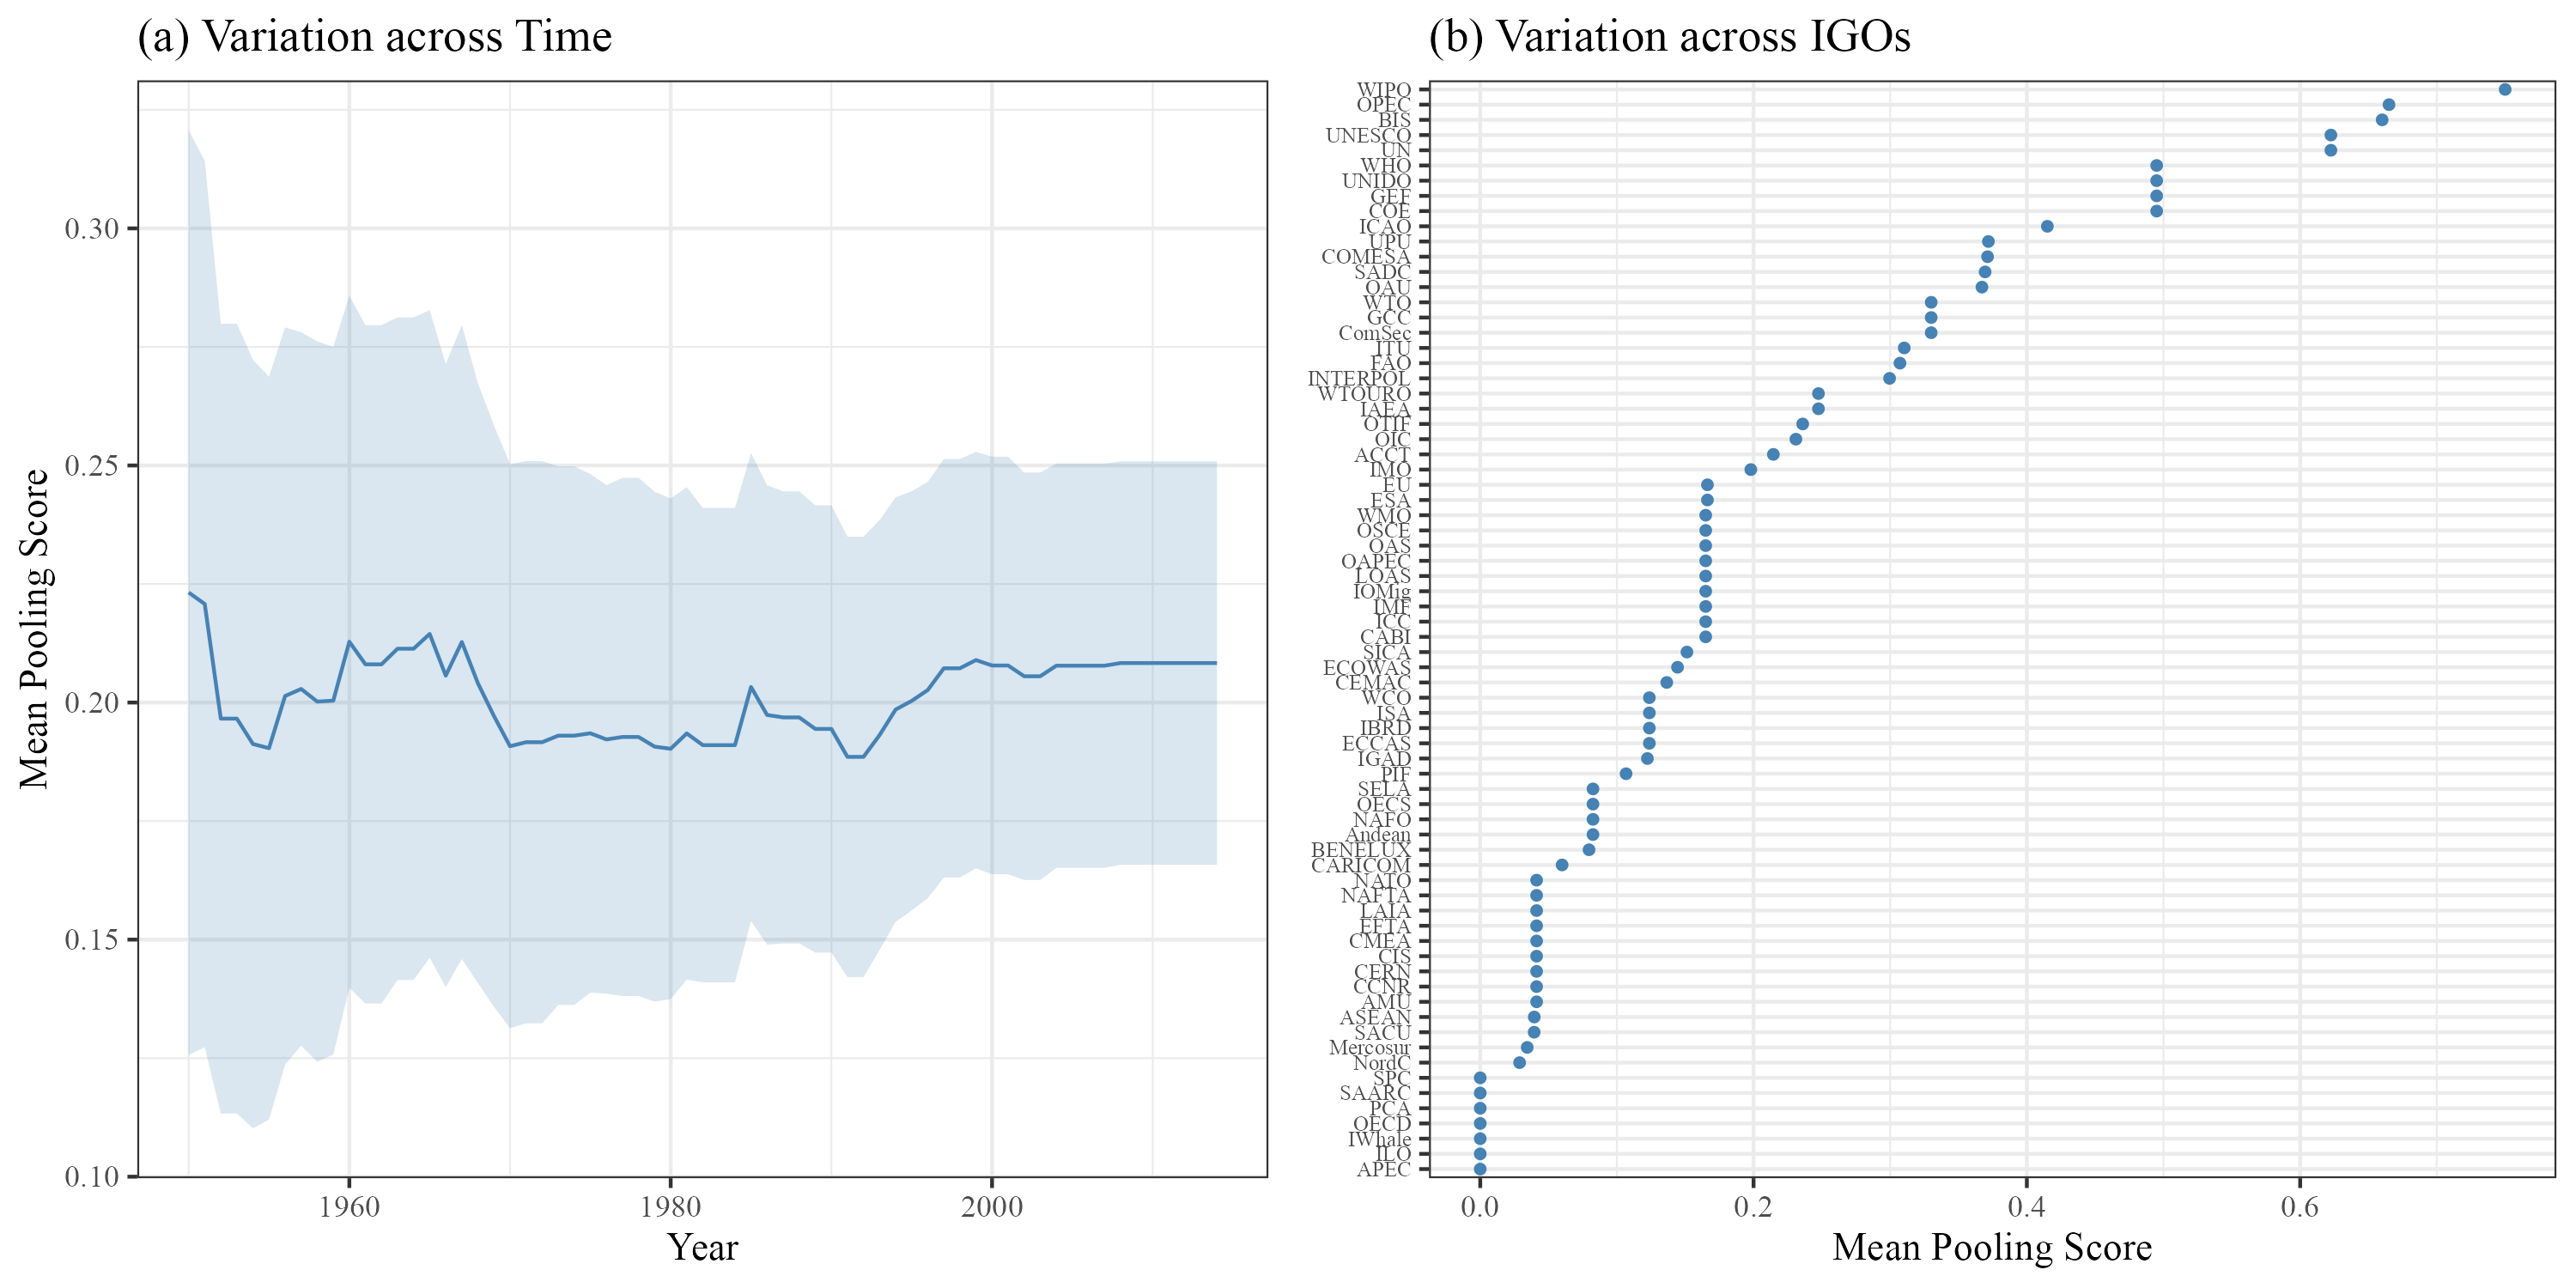
\includegraphics[width=\textwidth]{results/figure1_variation.png}

\caption{Variation in Amendment Flexibility Across Time and IGOs. Panel (a) plots the yearly average values of the constitutional pooling score from 1950 to 2020. Panel (b) shows cross-organizational variation in constitutional pooling, with notable heterogeneity in mean levels.}
\label{fig:variation}
\end{figure}

Figure~\ref{fig:variation} displays the variation in the constitutional pooling index across time and across IGOs. The left panel plots the yearly average values of constitutional pooling score, showing clear temporal variation. This indicates that IGOs' amendment flexibility is not static over time, supporting the use of a panel structure. The right panel demonstrates variation in constitutional pooling across individual IGOs, with notable heterogeneity in mean levels. Taken together, these figures provide empirical justification for panel modeling: the dependent variable varies both across time and across units, making a cross-sectional analysis (e.g., at the time of inception only) limited for capturing these dynamics.

Panel (a) shows that while the average pooling score remains relatively stable around 0.2 from 1950 to 2020, there is greater uncertainty in earlier years, as indicated by wider confidence intervals. Panel (b) reveals substantial cross-organizational variation. A few IGOs such as WIPO and the UN exhibit high pooling scores above 0.6, suggesting more flexible amendment procedures, while the majority cluster at much lower scores, with several IGOs, including Mercosur, ILO, and PCA, displaying low flexibility. This descriptive evidence highlights that amendment rules differ markedly across IGOs, while remaining largely stable within IGOs over time, consistent with the institutional stickiness of founding constitutional documents.

\section{Empirical Results and Discussion}

Using panel data at the IGO-year level, I estimate the relationship between IGO-level democracy and constitutional pooling. A higher pooling score indicates greater collective willingness to relinquish veto power over new amendments. Across all specifications, the results point in the same direction: more authoritarian IGOs consistently adopt more flexible amendment procedures.

\begin{figure}[H]
\centering
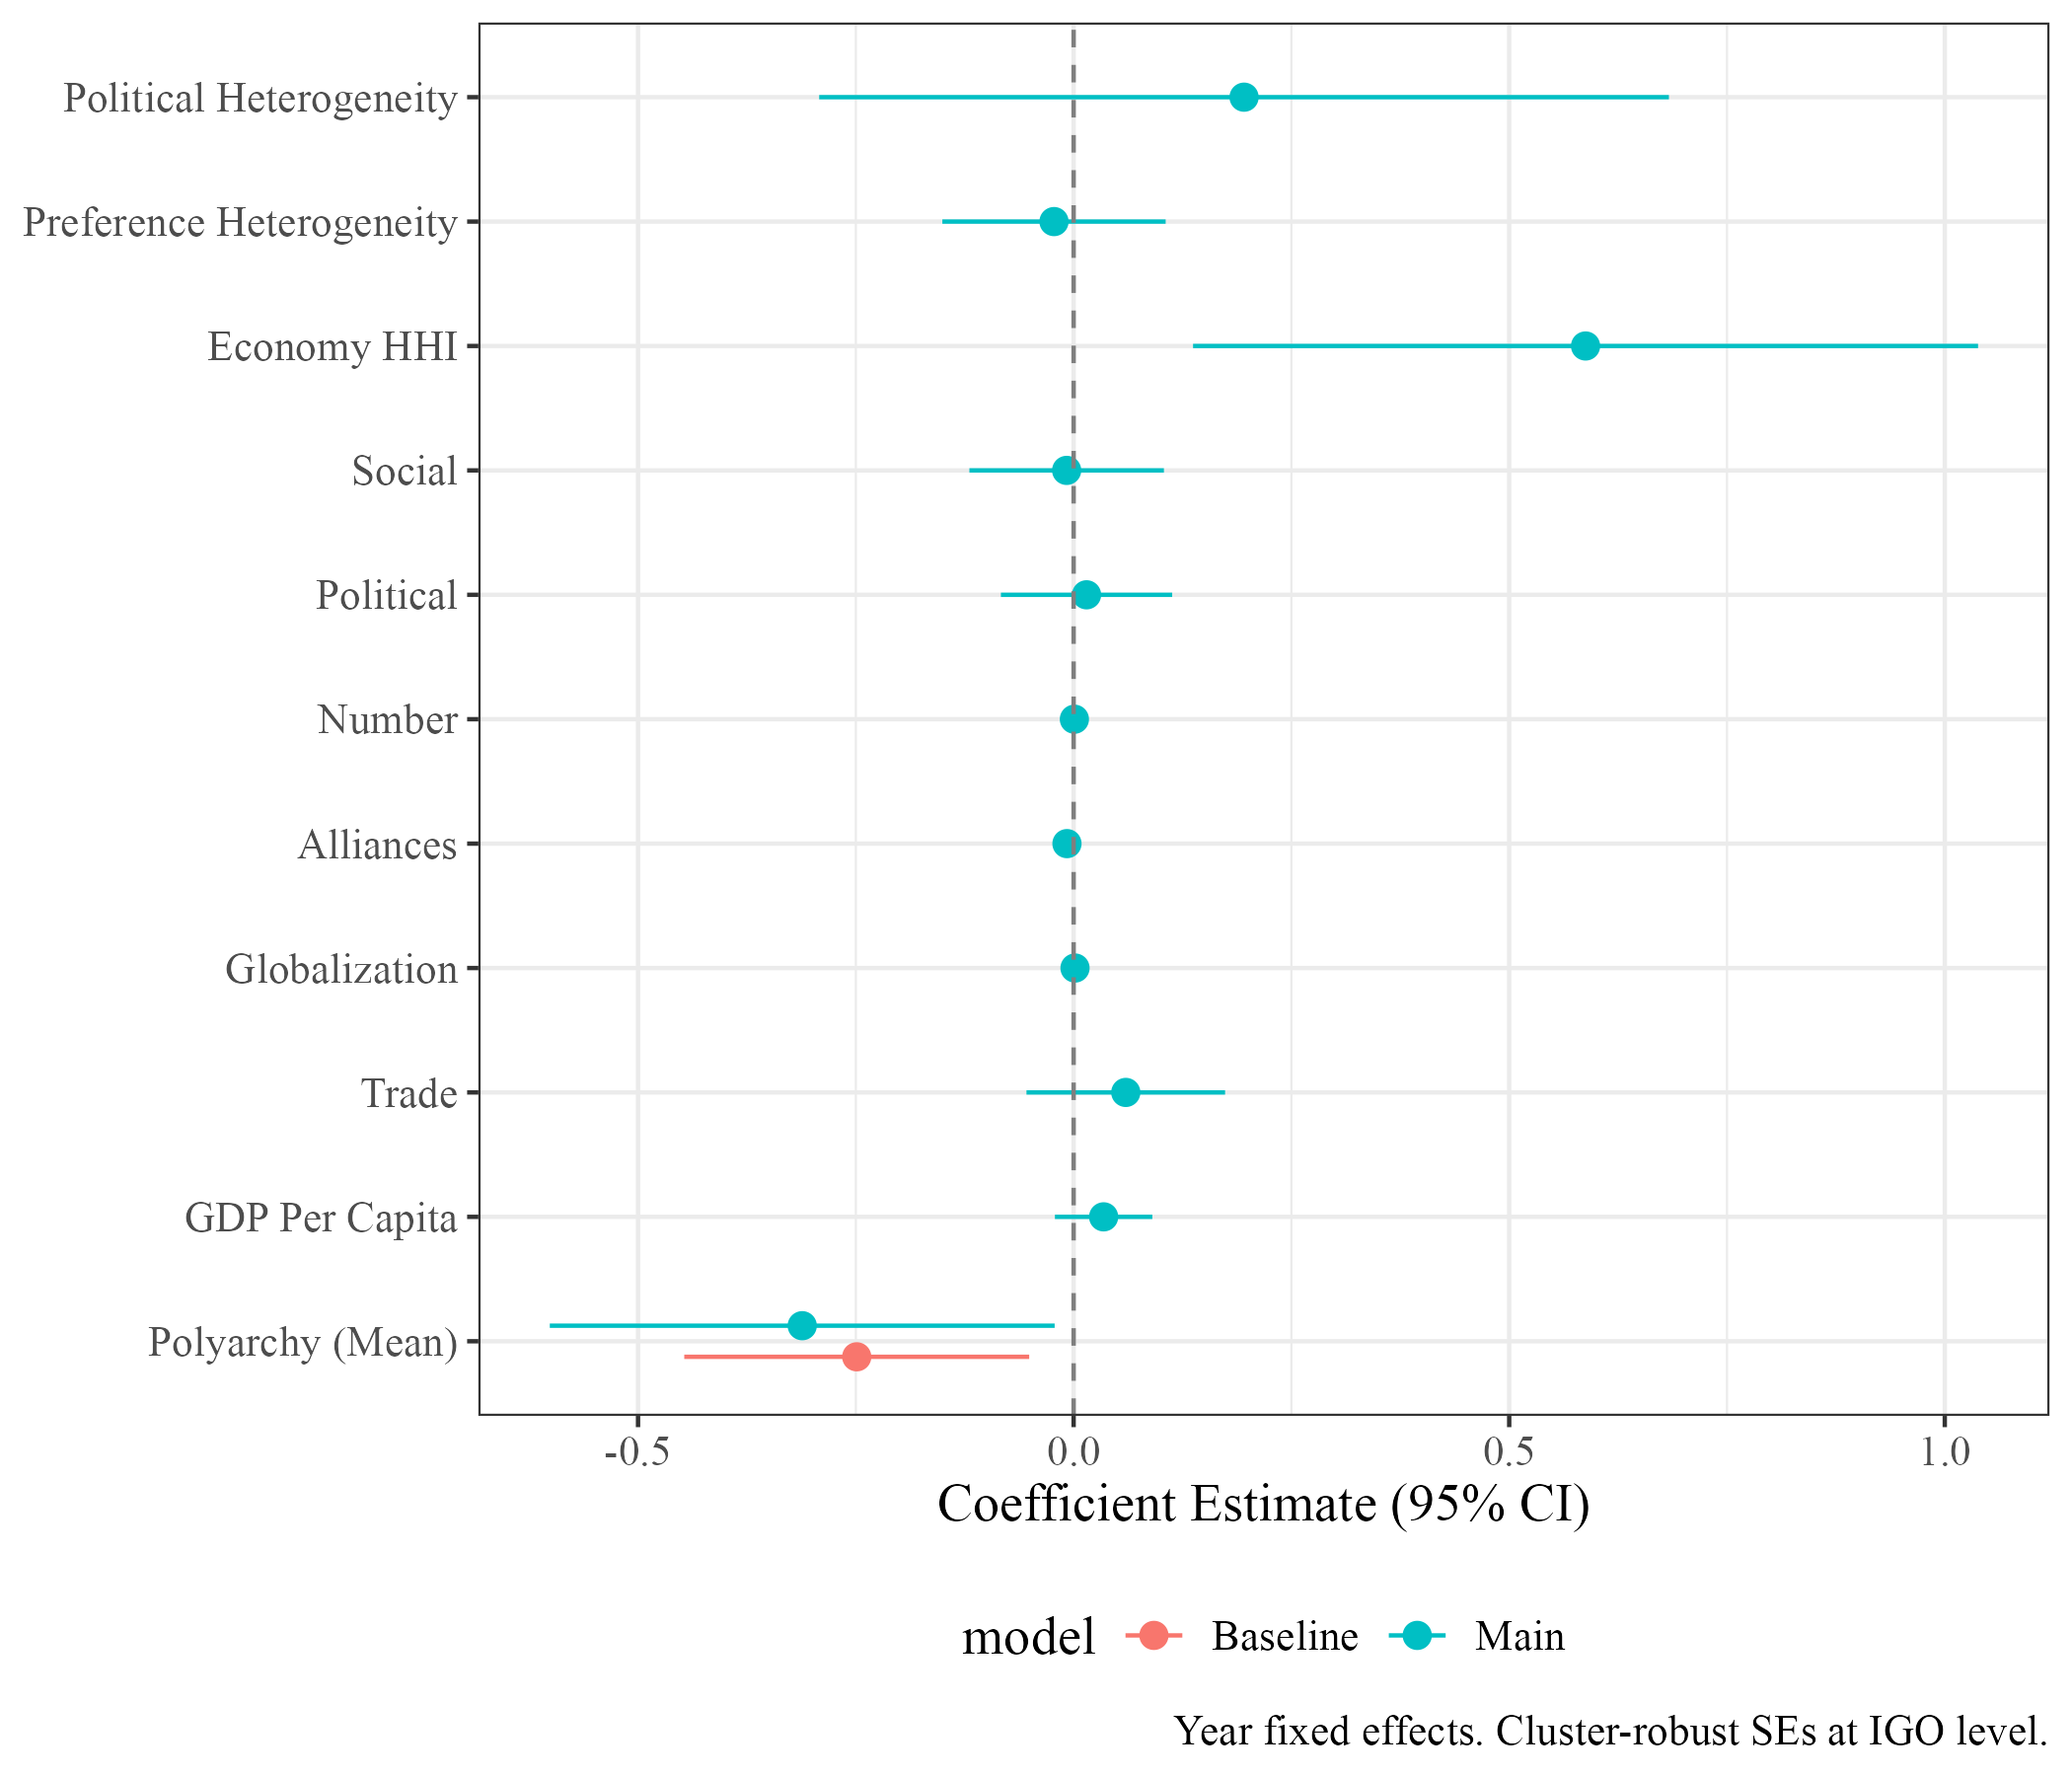
\includegraphics[width=0.85\textwidth]{results/main_coef_plot.png}
\caption{Coefficient estimates from a linear panel model examining the relationship between the average polyarchy score of an IGO's member states and constitutional pooling. Year fixed effects included. Cluster-robust standard errors at the IGO level.}
\label{fig:coef}
\end{figure}

Figure~\ref{fig:coef} and Appendix~\ref{app:coef_table} present coefficient estimates from the baseline and main specifications. The average polyarchy score of an IGO's member states is negatively associated with constitutional pooling and statistically significant at the $95\%$ confidence level. A one-unit increase in the average polyarchy score is associated with a 0.31 point decrease in the constitutional pooling score. Given that the pooling score ranges from 0 to 0.75 in the sample, this is a substantively meaningful effect. IGOs composed predominantly of authoritarian states are significantly more likely to institutionalize majority-based amendment procedures than their democratic counterparts.

Among the control variables, economic concentration within the IGO, measured by the Herfindahl-Hirschman index, is positively associated with pooling, as is organizational size. Alliance density is negatively associated with pooling, consistent with the expectation that IGOs whose members have many outside options place less value on internal flexibility. GDP per capita, trade openness, globalization, political and social purpose classification, and preference heterogeneity show limited effects across specifications and are not interpreted substantively here.

The main finding holds across alternative operationalizations of regime composition reported in Appendix~\ref{app:alterantive_rob}. Replacing the mean polyarchy score with the median, the percentage of democratic members, or the liberal democracy index yields substantively similar results, which reduces concern that the baseline finding is sensitive to how IGO-level democracy is measured. Tobit and hurdle model estimates reported in Appendices~\ref{app:tobit} and~\ref{app:hurdle} similarly confirm the negative relationship between authoritarian IGO composition and constitutional pooling at conventional significance levels, with somewhat larger point estimates than the OLS baseline. This pattern is consistent with the expectation that linear regression produces conservative estimates when the outcome is bounded and left-skewed. The linear model is retained as the main specification because its coefficients are directly interpretable and comparable to existing work on IGO institutional design procedures.




\section{Conclusion}

This paper addresses an important puzzle for both legal scholars and political scientists: Why would authoritarian governments, often seen as defenders of sovereignty and opponents of international legal constraint, voluntarily give up veto power over constitutional amendments? This is an underexplored intersection of international law, institutional design, and authoritarian politics. While conventional wisdom suggests that authoritarian states would cling to unanimity rules to preserve control, this study finds that autocracies, when cooperating with like-minded regimes, are more likely to adopt majority-rule frameworks. This counterintuitive finding highlights how lower external political costs and shared regime interests allow authoritarian states to prioritize flexibility over control. 

This finding has broader implications for the study of global governance. First, it challenges the intuition that democracy facilitates deeper international cooperation. In certain institutional domains, such as amendment flexibility, authoritarian regimes may be more willing to forgo domestic authority, as long as the institutional environment reflects their preferences and shields them from external interference.

Second, the findings suggest a need to rethink the strategic behavior of autocracies in international organizations. Rather than merely obstructing or deflecting cooperation, authoritarian states may actively shape institutional rules to serve their interests, facilitating faster adaptation, controlling revision procedures, and limiting external scrutiny.

Third, this paper underscores the importance of moving beyond aggregate measures of institutional design toward fine-grained theoretical frameworks and hypothesis testing that focus on specific institutional domains. Much of the existing literature treats pooling or delegation as broad, umbrella concepts that encompass a wide range of institutional features, ranging from voting procedures for policy decisions to rules governing new member accession or dispute settlement. While useful for general comparisons, these aggregate indicators can obscure the distinct political logics that operate in different functional areas of institutional design. In contrast, this paper's focus on amendment flexibility---rules governing how constitutional change occurs within IGOs---offers a more precise lens through which to observe strategic calculations by authoritarian states. By isolating this specific design feature, the analysis reveals a clear and consistent pattern: authoritarian regimes are more likely to endorse flexible, majority-based procedures for constitutional reform, particularly when embedded in ideologically aligned institutional environments. As such, the paper calls for greater theoretical and empirical attention to domain-specific variation in institutional rules, and how distinct elements of organizational design reflect the unique preferences, constraints, and power calculations of their member states. Future research could supplement these findings with case studies to further unpack the political calculations behind authoritarian cooperation in IGO governance.

\printbibliography

%------------------------------------------------------------
% APPENDIX
%------------------------------------------------------------
\appendix


\section{Stability}
\begin{table}[H]
\centering
\label{app:stability}
\begin{table}
\centering
\begin{talltblr}[         %% tabularray outer open
caption={Within-IGO Stability of Constitutional Pooling Rules},
]                     %% tabularray outer close
{                     %% tabularray inner open
colspec={Q[]Q[]Q[]Q[]Q[]},
hline{2}={1-5}{solid, black, 0.05em},
hline{1}={1-5}{solid, black, 0.1em},
hline{3}={1-5}{solid, black, 0.1em},
column{1-5}={}{halign=l},
}                     %% tabularray inner close
Total IGOs & IGOs with no change & IGOs with change & Pct. never changed & Mean obs. per IGO \\
\num{76.00} & \num{51.00} & \num{25.00} & \num{67.10} & \num{47.20} \\
\end{talltblr}
\end{table}

\end{table}


\section{Coefficient Table}
\begin{table}[H]
\centering
\label{app:coef_table}
\begin{table}[h]
\centering
\caption{Constitutional Pooling and IGO Regime Composition}
\label{app:coef_table_main}
\begin{tblr}{
colspec={Q[]Q[]Q[]},
hline{1}={1-3}{solid, black, 0.1em},
hline{2}={1-3}{solid, black, 0.05em},
hline{27}={1-3}{solid, black, 0.05em},
hline{30}={1-3}{solid, black, 0.1em},
column{2-3}={halign=c},
column{1}={halign=l},
}
& Baseline & Main \\
Polyarchy (Mean) & \num{-0.249}* & \num{-0.312}*** \\
& (\num{0.101}) & (\num{0.027}) \\
GDP Per Capita &  & \num{0.034}*** \\
&  & (\num{0.006}) \\
Trade &  & \num{0.060}*** \\
&  & (\num{0.018}) \\
Globalization &  & \num{0.002}*** \\
&  & (\num{0.000}) \\
Alliances &  & \num{-0.008}*** \\
&  & (\num{0.002}) \\
Number &  & \num{0.001}*** \\
&  & (\num{0.000}) \\
Political &  & \num{0.015}+ \\
&  & (\num{0.008}) \\
Social &  & \num{-0.008} \\
&  & (\num{0.009}) \\
Economy HHI &  & \num{0.588}*** \\
&  & (\num{0.062}) \\
Preference Heterogeneity &  & \num{-0.023} \\
&  & (\num{0.017}) \\
Political Heterogeneity &  & \num{0.196}** \\
&  & (\num{0.071}) \\
Num.Obs. & \num{3033} & \num{2678} \\
R2 & \num{0.067} & \num{0.270} \\
R2 Adj. & \num{0.050} & \num{0.255} \\
\end{tblr}
\footnotesize{+ p < 0.1, * p < 0.05, ** p < 0.01, *** p < 0.001} \\
\footnotesize{Year fixed effects. Cluster-robust SEs at IGO level.}
\end{table}
\end{table}

\section{Robustness Checks: Alternative Democracy Measures}
\begin{table}[H]
\centering
\label{app:alterantive_rob}
\centering
\begin{talltblr}[         %% tabularray outer open
caption={Robustness: Alternative Democracy Measures},
label={app:alterantive_rob},
note{}={+ p \num{< 0.1}, * p \num{< 0.05}, ** p \num{< 0.01}, *** p \num{< 0.001}},
note{ }={Year fixed effects. Cluster-robust SEs at IGO level.},
]                     %% tabularray outer close
{                     %% tabularray inner open
colspec={Q[]Q[]Q[]Q[]},
hline{2}={1-4}{solid, black, 0.05em},
hline{28}={1-4}{solid, black, 0.05em},
hline{1}={1-4}{solid, black, 0.1em},
hline{31}={1-4}{solid, black, 0.1em},
column{2-4}={}{halign=c},
column{1}={}{halign=l},
}                     %% tabularray inner close
& LibDem & Polyarchy & Percentage \\
Percentage of Democracy &  &  & \num{-0.174}* \\
&  &  & (\num{0.087}) \\
Liberal Democracy & \num{-0.332}* &  &  \\
& (\num{0.167}) &  &  \\
GDP Per Capita & \num{0.042} & \num{0.033} & \num{0.036} \\
& (\num{0.032}) & (\num{0.029}) & (\num{0.030}) \\
Trade & \num{0.065} & \num{0.061} & \num{0.046} \\
& (\num{0.058}) & (\num{0.057}) & (\num{0.061}) \\
Globalization & \num{0.001} & \num{0.001} & \num{0.001} \\
& (\num{0.001}) & (\num{0.001}) & (\num{0.001}) \\
Alliances & \num{-0.008}* & \num{-0.006}* & \num{-0.007}* \\
& (\num{0.003}) & (\num{0.003}) & (\num{0.003}) \\
Number & \num{0.001}* & \num{0.001}+ & \num{0.001}* \\
& (\num{0.000}) & (\num{0.000}) & (\num{0.000}) \\
Political & \num{0.014} & \num{0.009} & \num{0.013} \\
& (\num{0.051}) & (\num{0.051}) & (\num{0.049}) \\
Social & \num{-0.007} & \num{-0.012} & \num{-0.009} \\
& (\num{0.057}) & (\num{0.058}) & (\num{0.057}) \\
Economy HHI & \num{0.610}** & \num{0.598}** & \num{0.590}* \\
& (\num{0.228}) & (\num{0.232}) & (\num{0.237}) \\
Preference Heterogeneity & \num{-0.021} & \num{-0.017} & \num{-0.040} \\
& (\num{0.065}) & (\num{0.065}) & (\num{0.071}) \\
Political Heterogeneity & \num{0.160} & \num{0.239} & \num{0.254} \\
& (\num{0.240}) & (\num{0.272}) & (\num{0.273}) \\
Polyarchy (Median) &  & \num{-0.225}+ &  \\
&  & (\num{0.123}) &  \\
Num.Obs. & \num{2678} & \num{2678} & \num{2678} \\
R2 & \num{0.267} & \num{0.262} & \num{0.266} \\
R2 Adj. & \num{0.252} & \num{0.246} & \num{0.250} \\
\end{talltblr}

\end{table}


\section{Tobit Models}
\begin{table}[H]
\centering
\label{app:tobit}
\begin{table}
\centering
\begin{talltblr}[         %% tabularray outer open
caption={Robustness: Tobit Models (Left-Censored at 0)},
label={app:tobit},
note{}={+ p \num{< 0.1}, * p \num{< 0.05}, ** p \num{< 0.01}, *** p \num{< 0.001}},
note{ }={Tobit models with left-censoring at 0 and right-censoring at 1. Addresses bounded DV distribution.},
]                     %% tabularray outer close
{                     %% tabularray inner open
colspec={Q[]Q[]},
hline{2}={1-2}{solid, black, 0.05em},
hline{24}={1-2}{solid, black, 0.05em},
hline{1}={1-2}{solid, black, 0.1em},
hline{25}={1-2}{solid, black, 0.1em},
column{2}={}{halign=c},
column{1}={}{halign=l},
}                     %% tabularray inner close
& Polyarchy \\
Polyarchy (Mean) & \num{-0.336}*** \\
& (\num{0.029}) \\
GDP Per Capita & \num{0.033}*** \\
& (\num{0.006}) \\
Trade & \num{0.073}*** \\
& (\num{0.017}) \\
Globalization & \num{0.002}*** \\
& (\num{0.000}) \\
Alliances & \num{-0.008}*** \\
& (\num{0.002}) \\
Number & \num{0.001}*** \\
& (\num{0.000}) \\
Political & \num{0.008} \\
& (\num{0.009}) \\
Social & \num{-0.006} \\
& (\num{0.010}) \\
Economy HHI & \num{0.639}*** \\
& (\num{0.070}) \\
Preference Heterogeneity & \num{-0.028} \\
& (\num{0.019}) \\
Political Heterogeneity & \num{0.084} \\
& (\num{0.079}) \\
Num.Obs. & \num{2678} \\
\end{talltblr}
\end{table}

\end{table}

\section{Hurdle Model}
\begin{table}[H]
\centering
\label{app:hurdle}
\begin{table}
\centering
\begin{talltblr}[         %% tabularray outer open
caption={Robustness: Hurdle Model},
label={app:hurdle},
note{}={+ p \num{< 0.1}, * p \num{< 0.05}, ** p \num{< 0.01}, *** p \num{< 0.001}},
note{ }={Stage 1 models whether an IGO has any amendment flexibility (logit). Stage 2 models the degree of flexibility conditional on being nonzero (OLS). Robust standard errors.},
]                     %% tabularray outer close
{                     %% tabularray inner open
colspec={Q[]Q[]Q[]},
hline{2}={1-3}{solid, black, 0.05em},
hline{24}={1-3}{solid, black, 0.05em},
hline{1}={1-3}{solid, black, 0.1em},
hline{26}={1-3}{solid, black, 0.1em},
column{2-3}={}{halign=c},
column{1}={}{halign=l},
}                     %% tabularray inner close
& Stage 1: Any Flexibility (Logit) & Stage 2: Degree of Flexibility (OLS) \\
Polyarchy (Mean) & \num{-5.827}*** & \num{-0.262}*** \\
& (\num{0.704}) & (\num{0.024}) \\
GDP Per Capita & \num{0.493}*** & \num{0.034}*** \\
& (\num{0.130}) & (\num{0.005}) \\
Trade & \num{1.983}*** & \num{0.024}+ \\
& (\num{0.312}) & (\num{0.013}) \\
Globalization & \num{0.028}*** & \num{0.001}*** \\
& (\num{0.008}) & (\num{0.000}) \\
Alliances & \num{-0.129}*** & \num{-0.005}*** \\
& (\num{0.018}) & (\num{0.001}) \\
Number & \num{0.007}*** & \num{0.001}*** \\
& (\num{0.001}) & (\num{0.000}) \\
Political & \num{-0.294} & \num{0.026}** \\
& (\num{0.181}) & (\num{0.008}) \\
Social & \num{0.093} & \num{-0.002} \\
& (\num{0.188}) & (\num{0.009}) \\
Economy HHI & \num{1.314} & \num{0.588}*** \\
& (\num{1.541}) & (\num{0.044}) \\
Political Heterogeneity & \num{-7.333}*** & \num{0.317}*** \\
& (\num{1.708}) & (\num{0.067}) \\
Preference Heterogeneity & \num{-0.552}* & \num{0.001} \\
& (\num{0.261}) & (\num{0.019}) \\
Num.Obs. & \num{2678} & \num{2356} \\
R2 &  & \num{0.304} \\
\end{talltblr}
\end{table}

\end{table}

\end{document}